\documentclass{scrartcl}
\usepackage{etex}
\include{header/zusammenfassung}
\include{header/hyperref}
\include{header/listings}
\usepackage{tikz}
\usepackage{adjustbox}
\usetikzlibrary{arrows}
\usetikzlibrary{calc}
\usetikzlibrary{matrix}
\usetikzlibrary{intersections}

\newcommand\numberthis{\addtocounter{equation}{1}\tag{\theequation}}

\usepackage{circuitikz}
\usepackage{esdiff}

\tikzstyle{3x3mask}=[
	matrix of nodes, 
	nodes={draw, minimum size=8mm, anchor=center},
	column sep=0mm
]


% Spaltenabstand bei ,ulticols
\setlength{\columnsep}{1.5em}

\title{OrdDiff Zusammenfassung}
\subtitle{Dozent: Ch. Zaugg, Ordinary Differential Equation}
\author{Ch. Winterhalter, S. Malacarne, H. Diethelm}

\begin{document}
\selectlanguage{ngerman}

\lstset{language=Matlab}

\maketitle
\newpage

\tableofcontents
\newpage


\setcounter{section}{0}
%\input{sections/ImageSegmentation}
%\input{sections/RepresentationDescription}
%\input{sections/ObjectRecognition}
%\input{sections/PracticalExercises}

\section{Kappitel 1}

\subsection{Symbolisch}

\subsubsection{Allgemein 1. Ordnung}
$\dfrac{d}{dt}y(t)=f(t,y(t))$

\subsubsection{Linear DGL}
\begin{tabular}{p{6cm}p{2cm}p{10.5cm}}
\textbf{Form:} $y'(t) + p(t) \cdot y(t) = g(t)$ &
\textbf{Vorgehen:}              &

1. $\mu(t)$ berechnen: $\mu(t) = e^{\int p(t) dt}$ \\ &&
2. L"osung: $y(t) = \frac{1}{\mu(t)} \cdot ( \int \mu(t) g(t) dt +c)$ \\ &&
\end{tabular}
\textbf{Bsp}: $t^3 \cdot y'(t) + 4 t^2 \cdot y(t) = e^{-t} \quad \Longrightarrow \quad y'(t) + \underbrace{4 \frac{1}{t}}_{p(t)} \cdot y(t) = \underbrace{\frac{1}{t^3} e^-t}_{g(t))}$

\subsubsection{Separierbar DGL}
\begin{tabular}{p{6cm}p{2cm}p{10.5cm}}
\textbf{Form:} $M(x) + N(y(x))\cdot y'(x) = 0$ &
\textbf{Vorgehen:}              &

1. $H_1(x)$ berechnen: $H_1(x) = \int M(x) dx$ \\ &&
2. $H_2(y)$ berechnen: $H_2(y) = \int N(y)dy$ \\ &&
3. L"osung: $H_1(x) + H_2(y) = c$ ; c folgt aus Anf. Bed.\\\\
\end{tabular}
\textbf{Bsp}: $y'(x) = (1-2x)y^2 \quad \Longrightarrow \quad \underbrace{-(1-2x)}_{M(x)} + \underbrace{\frac{1}{y^2}}_{N(y(x))} \cdot y'(x) = 0$

\subsubsection{Exakte DGL}
\begin{tabular}{p{6cm}p{2cm}p{10.5cm}}
\textbf{Form:} $M(x,y) + N(x,y)\cdot y'(x) = 0$ &
\textbf{Vorgehen:}              &

1. Kompatibilitaets Bed. pr"ufen: $\diffp{M(x,y)}{y} = \diffp{N(x,y)}{x}$ \\ &&
2. $ M(x,y) = \dfrac{d}{dx}\Psi(x,y) \qquad N(x,y) = \dfrac{d}{dy}\Psi(x,y) $ \\ &&
3. $Q(x,y)$ berechnen: $Q(x,y) = \int M(x,y) dx$ \\ &&
4. $\diffp{h(y)}{y}$ berechnen: $\diffp{h(y)}{y} = N(x,y) - \diffp{Q(x,y)}{y}$ \\ &&
5. $h(y)$ berechnen: $h(y) = \int \diffp{h(y)}{y} dy $ \\ &&
6. L"osung: $\Psi(x,y) = Q(x,y) + h(y) = c $ \\ &&
\end{tabular}
\textbf{Bsp}: $(9x^2 + y -1)dx - (4y -x)dy = 0 \quad \Longrightarrow \quad  \underbrace{9x^2 +y -1}_{M(x,y)} + \underbrace{(-(4y -x))}_{N(x,y)} \cdot \diffp{y}{x} = 0$

%\subsubsection{Linear}
%
%\textbf{Form:} $\dfrac{d}{dt}y(t) +p(t)y(t)=g(t)$ \\
%
%\textbf{Vorgehen:}
%\begin{enumerate}
%\item $\mu(t)=e^{\int p(t)dt}$
%\item $y(t)=\dfrac{1}{\mu(t)}\left(\int{\mu(t)g(t) dt+C}\right)$
%\end{enumerate}
%
%
%\subsubsection{Separierbar}
%
%\textbf{Form:} $M(x)+N(y(x))(\dfrac{d}{dx}y(x))=0$\\
%
%\textbf{Vorgehen:}
%\begin{enumerate}
%\item $H_1=\int M(x)dx \qquad H_2=\int N(y)dy$
%\item $H_1(x) + H_2(y(x)) = C$
%\end{enumerate}
%
%\subsubsection{Exakt}
%\textbf{Form:} $M(x,y) + N(x,y)(\dfrac{d}{dx}y(x))=0$ 
%\quad wobei \quad $\dfrac{d}{dy}M(x,y) = \dfrac{d}{dx}N(x,y)$\\
%
%\textbf{Vorgehen:}
%\begin{enumerate}
%\item $ M(x,y) = \dfrac{d}{dx}\Psi(x,y) \qquad N(x,y) = \dfrac{d}{dy}\Psi(x,y) $
%\item Potential $\Psi(x,y) = Q(x,y) + h(y) \qquad Q(x,y) = \int M(x,y) dx$
%\item $\dfrac{d}{dy}h(y) = N(x,y) - \dfrac{d}{dy}Q(x,y) \rightarrow h(y)=\int dy$
%\item Lösung: $\Psi(x,y) = Q(x,y) + h(y) = c$
%\end{enumerate}


\subsection{Nummerisch}
\subsubsection{Fehler}

\begin{tabbing}
Tatzächlicher Wert  \= $\phi(t_n)$ \\
Globaler Fehler \> $E_n = \phi(t_n) - y_n$ \\
Lokaler Fehler \> $e_{n+1} = \phi(t_n + h) - y_{n+1}$ \\
Rundungsfehler \> $R_n = y_n - Y_n$ wobei $Y_n$ gerundet
\end{tabbing}

\subsubsection{Euler}
Polygonzug mit Steigung $y'(t)$\\
$y'(t)=f(t,y(t)) \qquad y(t_0)=y_0 \qquad$ Zeitschritt $h$\\
$t_i = t_{i-1} + h \qquad y_i=y_{i-1} + h \cdot f(t_{i-1},y_{i-1})$\\

$|\phi''(t)|<M \qquad |e_n| < \dfrac{M*h^2}{2} \qquad
h_n < \sqrt{\dfrac{2\epsilon}{M}} \qquad E_n \approx h$
\subsubsection{Heun}
Trapez Approximation\\
$y'(t)=f(t,y(t)) \qquad y(t_0)=y_0 \qquad$ Zeitschritt $h$\\
Idee: $y_i=y_{i-1} + h \cdot \dfrac{f(t_{i-1},y_{i-1}) + f(t_{i},y_{i})}{2}$\\
$t_i = t_{i-1} + h \qquad y_{i-1} + h \cdot \dfrac{f(t_{i-1},y_{i-1}) + f(t_{i},y_{i-1} + h \cdot f(t_{i-1},y_{i-1}))}{2}$\\
$e_n \approx h^3 \qquad E_n \approx h^2$
\subsubsection{Runge-Kutta}
$y_{i+1}=y_i + h \cdot \dfrac{k_{i,1} + 2\:k_{i,2} + 2\:k_{i,3} + k_{i,4} }{6}$\\
$k_{i,1} = f(t_{i},y_{i}) \qquad 
k_{i,2} = f(t_{i} + \dfrac{h}{2},y_{i} + \dfrac{h}{2}k_{i,1}) \qquad 
k_{i,3} = f(t_{i} + \dfrac{h}{2},y_{i} + \dfrac{h}{2}k_{i,2}) \qquad 
k_{i,3} = f(t_{i} + h,y_{i} + h \: k_{i,2}) \qquad$\\
$e_n \approx h^5 \qquad E_n \approx h^4$
\subsection{Bifurkationen}
Gegeben ist eine autonome Differentialgleichung mit reellen Parametern.

\begin{equation*}
	\diffp{}{t}y(t) = f(a,y(t))
\end{equation*}

Gesucht die Kritischen punkte die sogenannten Gleichgewichtslösungen. Diese sind wie folgt definiert:
\begin{equation*}
	\diffp{}{t}y(t) = 0
\end{equation*}
Die Gleichgewichtslösungen wird in 3 Fälle unterschieden:\\

\begin{minipage}[h]{0.35\textwidth} 
	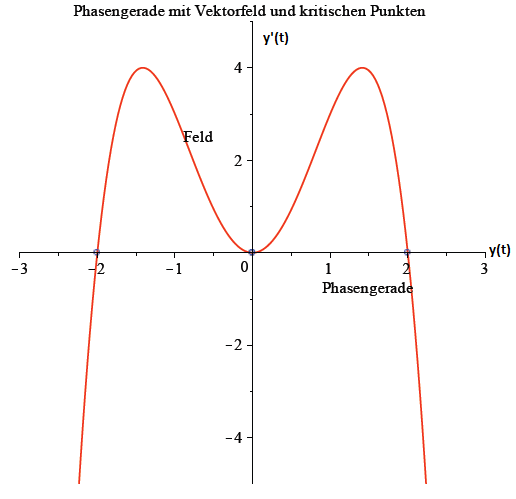
\includegraphics[width=1.0\textwidth]{images/Phasengerade.png}
\end{minipage}
\begin{minipage}[h]{0.35\textwidth}
	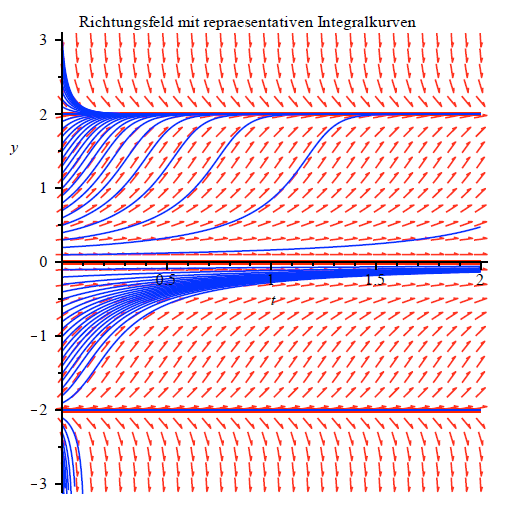
\includegraphics[width=1.0\textwidth]{images/Richtungsfeld.png}
\end{minipage}
\begin{tabular}{p{1.8cm}p{5cm}}
	$y(t) = -2$: & instabiel \\
	$y(t) = 0$: & semistabil\\
	$y(t) = 2$: & asymtotisch stabil\\
\end{tabular}

\section{Kapitel 2}

\subsection{Begriffe}
\subsubsection{Vektorfeld und Trajektorie}

\begin{tikzpicture}[>=latex]
    
    % Gleichung
    \node[anchor=west] at (8,6.5) {$x'(t) = f(t,x(t))$ \quad mit \quad $x(t_0)=x_0$};
    
    % Koordinatensystem
    \draw[thick,->] (0,0) -- (8,0) node[anchor=west] {$t$};
    \draw[thick,->] (0,0) -- (0,6) node[anchor=south] {$x_2$};
    \draw[thick,->] (0,0) -- (3,4) node[anchor=south west] {$x_1$};
    \draw[thin,dotted]	 (2,2.67) -- (8,2.67) -- (6,0)
                        (0,3.5) -- (2,6.17) -- (8,6.17) -- (6,3.5) -- (0,3.5)
                        (2,2.67) -- (2,6.17)
                        (8,2.67) -- (8,6.17)
                        (6,0) -- (6,3.5)
    ;
    
    % Lösungskurve
    \draw[HSRBlue] 
        (0,0.5) node[draw,circle,inner sep=2pt,label={[label distance=0.5]180:$x_0$}]{} 
        cos
        (8,5) node[draw,circle,inner sep=2pt,label={[label distance=0.5]0:Lösungskurve $\{(t,\varphi(t)),t \in I\}$}] {}
    ;
    
    % Trajektorie
    \draw[HSRBlue,dashed] (0,0.5) cos (2,5) node[draw,solid,circle,inner sep=2pt]{};
    \draw (-2.2,3) node[anchor=south]{Trajektorie $\{ \varphi(t),t \in I \}$} -- (1,2.5);
    
    % Phasenraum
    \draw (2.2,6.5) node[anchor=south]{Phasenraum, $(x_1,x_2)$-Ebene} -- (1.9,5.8);
    \draw (3,-0.5) node[anchor=north]{Erweiterter Phasenraum, Zustandsraum, $(t,x_1,x_2)$-Raum} -- (2.7,0.3);
    
    % Punkt t
    \draw (4,-0.1) node[anchor=north] {\color{HSRHematite}$t$} -- (4,0.1);
    \draw[dotted,HSRHematite] (4,0) -- (4.5,1.5) -- (4.5,2.15) node[draw,fill,circle,inner sep=2pt] {};
    \node[draw,fill,circle,HSRHematite,inner sep=2pt] at (1.1,2.15) {};
    \draw[dotted,HSRHematite] (1.1,2.15) -- (4.5,2.15);
    
    \draw[very thick,->,HSRHematite] (4.5,2.15) -- (5.1,2.5) node[midway,anchor=north west]{Richtungsfeld $(1,f(t,x))$};
    \draw[very thick,->,HSRHematite] (1.1,2.15) -- (1.35,2.7) node[midway,anchor=west]{Vektorfeld $(f(t,x))$};

\end{tikzpicture}


\subsubsection{Richtungsfeld und Lösung - Begriff der Lösung}
Die Lösung der Differentialgleichung $\frac{d}{dt}x(t) = f(t,x(t))$ ist eine parametrisierte Kurve x(t). Die Ableitung nach t ist demnach der Tangentenvektor an diese Kurve. Die Diffgleichung enthält demnach die Information über die Tangentenvektoren an ihre Lösungskurven. 
Das bedeutet, auch ohne die Lösung können wir die rechte Seite der Gleichung - d.h. die Tangentenvektoren - zeichnen. Das Lösen der Gleichung ist schlussendlich nur das Einpassen von Kurven in dieses Vektorfeld. Solche Kurven sind die Trajektorien der Gleichung. Die Trajektorie ist jedoch \textbf{nicht} die Lösung, da als Beispiel die Zeitkomponente fehlt. Hätte man (t,x(t)), hätte man die gesamte Lösung. 
\begin{minipage}[h]{0.35\textwidth} 
	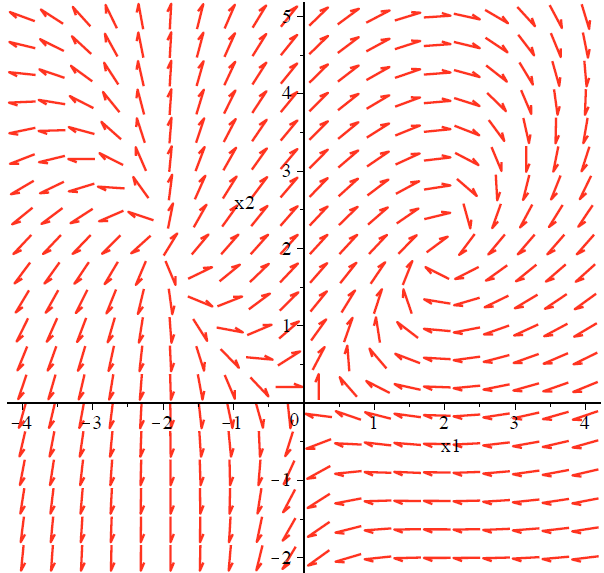
\includegraphics[width=0.9\textwidth]{images/Vektorfeld.png}
\end{minipage}
\begin{minipage}[h]{0.35\textwidth}
	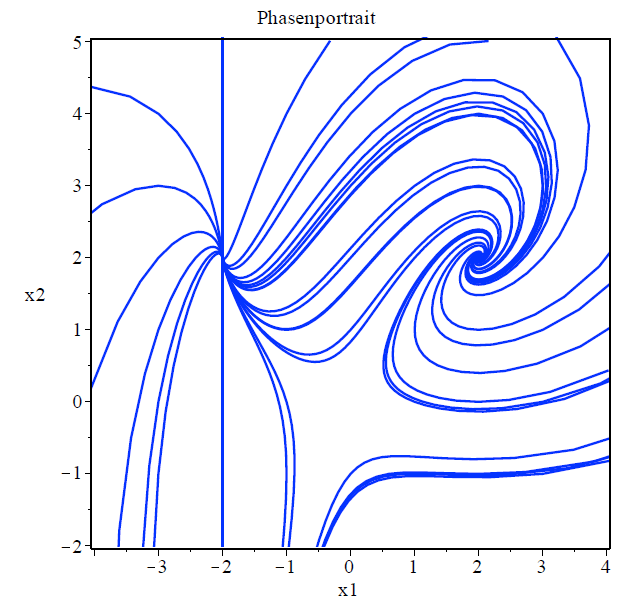
\includegraphics[width=1.0\textwidth]{images/Phasenportrait.png}
\end{minipage}

\subsection{Matrixdarstellung}
$x' = Ax + b$\\
Kritische Punkte: $x' = Ax + b = 0$ Gleichgewicht: $b = -Ax$ oder $x = -A^{-1}*b$\\
Lösungen bei b=0 (homogenen Gleichung): Für jeden Eigenwert und Eigenvektor eine Lösung: \\
$x_1(t) = e^{\lambda_1t}v_1,x_2(t) = e^{\lambda_2t}v_2...x_n(t) = e^{\lambda_nt}v_n$\\

\subsection{Variation der Konstanten}
Gegeben ist ein lineares, inhomogenes System 1. Ordnung: \\
\begin{equation*}
\frac{d}{dt}x(t) = Ax(t) + b(t) 
\end{equation*}
Als erstes werden die Lösungen der homogenen Gleichung gelöst, wir erhalten für jeden Eigenwert und Eigenvektor eine Lösung: \\
$x_1(t) = e^{\lambda_1t}v_1,x_2(t) = e^{\lambda_2t}v_2...x_n(t) = e^{\lambda_nt}v_n$\\
Diese Lösungen ergeben unsere Fundamentalmatrix:\\
\begin{equation*}
X(t) = 
	\begin{bmatrix} 
	        x_1(t) && x_2(t) && ... && x_n(t)\\    
	\end{bmatrix}
\end{equation*}

Mit Hilfe der Fundamentalmatrix können wir nun die partikuläre Lösung des Systems bestimmen:\\
\begin{equation*}
y_P(t) = X(t) \int{X(t)^{-1}b(t)dt}
\end{equation*}
Die gesamte Lösung ist nun die Summe der homogenen und der partikulären Lösung.

\newpage
\subsection{Superpositionsprinzip}
Gegeben ist folgendes lineares homogenes Gleichungssystem:
\begin{equation*}
\frac{d}{dt}x(t) = A(t)x(t)
\end{equation*}
Das Superpositionsprinzip sagt, dass die Linearkombination der beiden Lösungen $x_1(t)$ und $x_2(t)$ auch wieder eine Lösung des Differentialgleichungssystems ist. 
\begin{equation*}
	x(t) = c_1 x_1(t) + c_2 x_2(t)
\end{equation*}
Wobei $c_1$ und $c_2$ beliebige Skalare sind. 
Das Prinzip kann auch für Systeme höherer Ordnung verwendet werden. \\

Hier ein \textbf{Beispiel} für eine Differentialgleichung zweiter Ordnung: \\
Gegeben: $t^2y''(t)-4ty'(t)+6y(t)=0$, $t>0$, $y_1(t)=t^2$\\
Gesucht: Eine zweite Lösung $y_2(t)$, so dass ${y_1(t),y_2(t)}$ ein Fundamentalsystem ergeben. \\
Vorgehensweise: \\
\textbf{Schritt 1:}\\
Prüfen, ob $y_1(t)$ wirklich Lösung des Systems ist. \\
\textbf{Schritt 2:}\\
Für die zu bestimmende Lösung $y_2(t)$ kommt folgender Ansatz zum Zug: $y_2(t) = v(t)y_1(t)$.\\
\textbf{Schritt 3:}\\
Ansatz $v(t)y_1(t)$ in Differentialgleichung einsetzen. Die Gleichung so weit es geht umformen und danach nach $v(t)$ auflösen. Wenn $v(t)$ bekannt ist, kann $y_2(t)$ berechnet werden. \\
\textbf{Schritt 4:}\\
Auf Grund der beiden Lösungen, kann die Fundamentalmatrix $Y(t) =
\begin{vmatrix} 
	        y_{1}(t) & y_{2}(t)\\ 
	        y'_{1}(t) & y'_{2}(t)\\   
\end{vmatrix} $ berechnet werden und mit Hilfe der Wronskideterminante geprüft werden, ob die Lösungen linear unabhängig sind ($det(W) \neq 0$). 

\subsection{Lineare Unabhängigkeit}
Die lineare Unabhängigkeit der beiden Lösungen $x_1(t)$ und $x_2(t)$ kann mit Hilfe der \textbf{Wronskideterminante} geprüft werden. 
\begin{equation*}
	W(t) = det[X(t)] =    
	\begin{vmatrix} 
	        x_{11}(t) & x_{12}(t)\\ 
	        x_{21}(t) & x_{22}(t)\\   
	\end{vmatrix}
\end{equation*}
Sind $x_1(t)$ und $x_2(t)$ \textbf{linear unabhängig}, dann gilt $W(t) \neq 0$ für alle $t \in I$. \\
Sind $x_1(t)$ und $x_2(t)$ \textbf{linear abhängig}, dann gilt $W(t) = 0$ für alle $t \in I$. \\
Jede Lösung $\Phi(t)$ kann als Linearkombination eines Fundamentalsystems zweier Lösungen $x_1(t)$ und $x_2(t)$ dargestellt werden. Diese Linearkombination wird als die allgemeine Lösung eines linearen homogenen Systems bezeichnet. \\
\textbf{Theorem von Abel}\\
\begin{equation*}
W(t) = c\cdot e^{\int{\operatorname{trace}(A(t))dt}}
\end{equation*}
Spur einer Matrix = Summe der Hauptdiagonalelemente
\subsection{Fluss eines Vektorfeldes}
Die Matrix A ordnet jedem Vektor x einen Vektor A(x) des Vektorfeldes zu. Der Fluss $\Phi(t)$ transformiert jeden Anfangszustand $x_0$ längs der druch $x_0$ verlaufenden Trajektorie in den Zustand x(t) zur Zeit t. \\
Es gelten folgende Zusammenhänge:\\
\begin{equation*}
\Phi(t) = X(t)X(t_0)^{-1}
\end{equation*}

\begin{equation*}
\Phi(t)X(t_0) = X(t)
\end{equation*}

\begin{equation*}
\Phi'(t) = A(t)\Phi(t)
\end{equation*}

\begin{equation*}
\Phi(t_0) = E
\end{equation*}

\begin{equation*}
\Phi(t) = e^{A(t)t} =\sum_{k=0}^{\infty}\frac{(A(t)\cdot t)^k}{k!}
\end{equation*}

Beispiele:\\
Gegeben: $A = 	\begin{vmatrix} 
	        		\lambda & 0\\ 
	        		0 & \lambda\\   
				\end{vmatrix} 
				\rightarrow$ 
$e^{tA} = \begin{vmatrix} 
	        		e^{t\lambda} & 0\\ 
	        		0 & e^{t\lambda}\\   
				\end{vmatrix}$\\
Gegeben: $A = 	\begin{vmatrix} 
	        		\lambda & 1\\ 
	        		0 & \lambda\\   
				\end{vmatrix} 
				\rightarrow$ 
$e^{tA} = \begin{vmatrix} 
	        		e^{t\lambda} & te^{t\lambda}\\ 
	        		0 & e^{t\lambda}\\   
				\end{vmatrix}$\\
				
Gegeben: $A = 	\begin{vmatrix} 
	        		2 & 3\\ 
	        		3 & 2\\   
				\end{vmatrix} \rightarrow
				\lambda_1=5 \; \lambda_2=-1 \rightarrow ev_1=\begin{vmatrix}
					1\\ 
					1\\   
				\end{vmatrix} \;
				ev_2=\begin{vmatrix}
					1\\ 
					-1\\   
				\end{vmatrix} \rightarrow
				T=\begin{vmatrix} 
	        		1 & 1\\ 
	        		1 & -1\\   
				\end{vmatrix} \rightarrow 
				B=T^{-1} \cdot A \cdot T=\begin{vmatrix} 
	        		5 & 0\\ 
	        		0 & -1\\   
				\end{vmatrix} \rightarrow$\\
				\hspace*{4cm}$e^{tA}=T \cdot e^{tB} \cdot T^{-1}=
				T \cdot \begin{vmatrix} 
					e^{5 t} & 0\\ 
					0 & e^{-t}\\   
				\end{vmatrix} \cdot T^{-1} =
				\dfrac{1}{2}\begin{vmatrix} 
					e^{5 t} + e^{-t}& e^{5 t} - e^{-t}\\ 
					e^{5 t} - e^{-t} & e^{5 t} + e^{-t}\\   
				\end{vmatrix}$


%Das Vektorfeld lässt sich auch aus dem Fluss zurück gwinnen, indem die Trajektorie $\phi(t) = \Phi(t)x$ nach er Zeit an der Stelle $t=0$ abgeleitet
%Gegeben ist ein autonomes lineares homogenes System mit einer nxn Matrix A:
%\begin{equation*}
%\frac{d}{dt}x(t) = A(t)x(t)
%\end{equation*}
%Die Matrix $A(t)$ besitzt verschiedene reelle Eigenwerte. Aus den Eigenwerten $\lambda_1$ und $\lambda_2$ und ihren zugehörigen Eigenvektoren $\nu_1$ und $\nu_2$ erhalten wir ein System von Fundamentallösungen: 
%\begin{equation*}
%x_1(t) = e^{\lambda_1t}\nu_1\\
%\end{equation*}
%\begin{equation*}
%x_2(t) = e^{\lambda_2t}\nu_2
%\end{equation*}
%Die Fundamentallösungen $x_1(t)$ und $x_2(t)$ bilden die Spalten der Fundamentalmatrix $X(t)$:
%\begin{equation*}
%	X(t) =     
%	\begin{vmatrix} 
%	        x_{11}(t) & x_{12}(t)\\ 
%	        x_{21}(t) & x_{22}(t)\\   
%	\end{vmatrix}
%\end{equation*}
%Diese Fundamentalmatrix genügt folgender Differentialgleichung: 
%\begin{equation*}
%\frac{d}{dt}X(t) = A(t)X(t)
%\end{equation*}
%Fluss? Versteh ich nicht so ganz. 
%
%Die Lösung x(t) des Anfangswertproblems $x(t_0) x_0$ kann mit Hilfe einer Fundamentalmatrix X(t) dargestellt werden. Die allgemeine Lösung der Diffgleichung $\frac{d}{dt}x(t) = A(t)x(t)$ kann als Superposition von Fundamentallösungen  geschrieben werden.\\
%\begin{equation*}
%x(t) = c_1 x_1(t) + ... + c_n x_n(t)
%\end{equation*}
%\begin{equation*}
%x(t) = X(t)c
%\end{equation*}
%Mit $x_0 = X(t_0)$ und $det(X(t_0)) \neq 0$
%\begin{equation*}
%c = X(t_0)^{-1}x_0
%\end{equation*}
%In obige Gleichung eingesetzt, ergibt: 
%\begin{equation*}
%x(t) = X(t)X(t_0)^{-1}x_0
%\end{equation*}
%Wählt man nun die Fundamentallösungen $x_1(t) ... x_n(t)$ zu den Anfangsbedingungen $x_1(t_0)=e_1, ..., x_n(t_0)=e_n$, wobei $e_1...e_n$ die kanonischen Basisvektoren des Vektorraumes $R^n$ sind, erhalten wir die zugehörige Fundamentalmatri:
%\begin{equation*}
%\Phi(t_0) = E
%\end{equation*}
%Es folt aus dem Eindeutigkeitssatz, dass die Lösung x(t) des Anfangswertproblems $x(t_0) = x_0$ mit Hilfe dieser speziellen Fundamentalmatrix $\Phi(t)$, folgende Darstellung besitzt: 
%\begin{equation*}
%x(t) = \Phi(t)x_0
%\end{equation*}
%mit $\Phi(t) = X(t)X(t_0)^{-1}$. In Worten: Die Matrix A ordnet jedem Vektor x einen Vektor A(x) des Vektorfeldes zu. Der Fluss $\Phi(t)$ transformiert jeden Anfangszustand $x_0$ längs der druch $x_0$ verlaufenden Trajektorie in den Zustand x(t) zur Zeit t. 
%Das Vektorfeld lässt sich auch aus dem Fluss zurück gwinnen, indem die Trajektorie $\phi(t) = \Phi(t)x$ nach er Zeit an der Stelle $t=0$ abgeleitet wird. 
%\begin{equation*}
%\frac{d}{dt}\Phi(t)x = A(x)
%\end{equation*}

\subsection{Matrixexponential}
Gegeben ist die Differentialgleichung:
\begin{equation*}
\frac{d}{dt}x(t) = A(t)x(t)
\end{equation*}
mit Anfangsbedingung $x(0) = x_0$ und der konstanten $n \times n$ Matrix A. Mit Hilfe des Flusses $\Phi(t)$ kann die Lösung dieses Problems dargestellt werden als: 
\begin{equation*}
x(t) = \Phi(t)x_0
\end{equation*}
Bei einer skalaren Differentialgleichung $\frac{d}{dt}x(t) = ax(t)$ ist die Lösung bei gegebener Anfangsbedingung: $x(t) = e^{at}x_0$. Wenn wir diese Lösung nun mit $\Phi(t)$ vergleichen, stellt sich heraus, dass der Fluss eines $n \times n$ Systems ebenfalls eine Exponentialdarstellung besitzt. 
Ist $A$ eine konstante $n \times n$ Matrix, dann besittz der Fluss $\Phi(t)$, der vom Vektorfeld erzeugt wird, folgende Darstellung als Matrixexponential: 
\begin{equation*}
\Phi(t) = e^{At} = X(t)X(0)^{-1}
\end{equation*}
Der Fluss wie auch das Matrixexponential können also mit Hilfe der Fundamentalmatrix X(t) und der entsprechenden Anfangsbedingung berechnet werden.
Damit hat die Lösung x(t) des Anfangswertproblems $x(0) = x_0$ folgende Form: 
\begin{equation*}
x(t) = e^{At}x_0
\end{equation*}


\subsection{Degenerierte Matrizen}
Ist $A$ degeneriert, bedeutet dies, dass sie mindestens einen Eigenwert $\lambda$ mit einer geometrischen Vielfachheit (Anzahl Eigenvektoren) besitzt, die kleiner als seine algebraische Vielfachheit (Anzahl gleiche Eigenwerte $m$) ist. 
Das bedeutet, dass die linear unabhängigen Eigenvektoren der Matrix $A$ den Raum $\mathbb{R}^n$ nicht ausschöpft.\\
Ist $\lambda$ ein Eigenwert von $A$ mit der algebraischen Vielfachheit $m$, dann besitzt die Gleichung: 
\begin{equation*}
(A-\lambda E)^m b_k = 0
\end{equation*}
eine Anzahl $m$ linear unabhängige Lösungen $b_1$ bis $b_m$ und für $k = 1,\ldots,m$ sind die vektorwertigen Funktionen
\begin{equation*}
x_k(t) = e^{\lambda t}\left[{b_k + \frac{t}{1!}(A-\lambda E)b_k + ... + \frac{t^{m-1}}{(m-1)!}(A-\lambda E)^{m-1}b_k}\right]
\end{equation*}
\begin{equation*}
 \Longrightarrow x_k(t) = e^{\lambda t}(b_k + t (A-\lambda E) b_k))
\end{equation*}
linear unabhängige Lösungen der Differentialgleichung. 
\subsection{Beispiel}
Folgende Matrix A ist gegeben: 
\begin{equation*}
	A =     
\begin{bmatrix} %phantom is for spacing
	2 & 0 & -1\\
	0 & 3 & 1\\
	0 & 0 & 2\\
\end{bmatrix}
\end{equation*}
\begin{equation*}
\det(A-\lambda E) = 0 \qquad \Longrightarrow \lambda_1 = 2 \text{(Doppelt)} \quad \lambda_2 = -1
\end{equation*}

\textbf{Schritt 1:} Eigenvektoren berechenen (Hier im Beispiel nur für $\lambda_1$)\\
\begin{equation*}
(A - \lambda_1 E)\nu = 0 \qquad \Longrightarrow \nu = 
\begin{bmatrix} %phantom is for spacing
	1 \\
	0 \\
	0 \\
\end{bmatrix}
\end{equation*}


\begin{equation*}
\Longrightarrow \text{Nur ein Eigenvektor aber zwei Eigenwerte $\lambda_1 = 2$} \quad \Longrightarrow m = 2
\end{equation*}
\textbf{Schritt 2:} Basisvektorern $b_k$ bestimmen \\
\begin{equation*}
(A-\lambda E)^2 b_k = 0 \qquad \Longrightarrow 0\cdot b_{k1} + 9\cdot b_{k2} - 3\cdot b_{k3} = 0
\end{equation*}
\begin{equation*}
b_1= 
\begin{bmatrix} %phantom is for spacing
	1 \\
	0 \\
	0 \\
\end{bmatrix}
\qquad b_2= 
\begin{bmatrix} %phantom is for spacing
	0 \\
	1 \\
	3 \\
\end{bmatrix}
\end{equation*}
\textbf{Schritt 3:} Lösung bestimmen\\
\begin{equation*}
x_1(t) = e^{2 \cdot t} (b_1 + t(A -  2 E)b_1) \qquad \Longrightarrow e^{2\cdot t}
\begin{bmatrix} %phantom is for spacing
	1 \\
	0 \\
	0 \\
\end{bmatrix}
\end{equation*}
\begin{equation*}
x_2(t) = e^{2 \cdot t} (b_2 + t(A -  2  E)b_2) \qquad \Longrightarrow e^{2\cdot t}
\begin{bmatrix} %phantom is for spacing
	-3t \\
	1 \\
	3 \\
\end{bmatrix}
\end{equation*}
\begin{equation*}
 \Longrightarrow X(t) = 
\begin{bmatrix} %phantom is for spacing
	 x_1(t) & x_2(t) \\
\end{bmatrix}
=
\begin{bmatrix} %phantom is for spacing
	1 \cdot e^{2 \cdot t} & -3t \cdot e^{2 \cdot t} \\
	0 & 1\cdot e^{2 \cdot t}  \\
	0 & 3 \cdot e^{2 \cdot t} \\
\end{bmatrix}
\end{equation*}


\subsection{Stabilit"at linearer Systeme}


\subsection{Entkoppeln}
\begin{minipage}[h]{0.35\textwidth}
Doppelter reeller Eigenwert:\\ Entkoppeln
\end{minipage}
\begin{minipage}[h]{0.5\textwidth}
	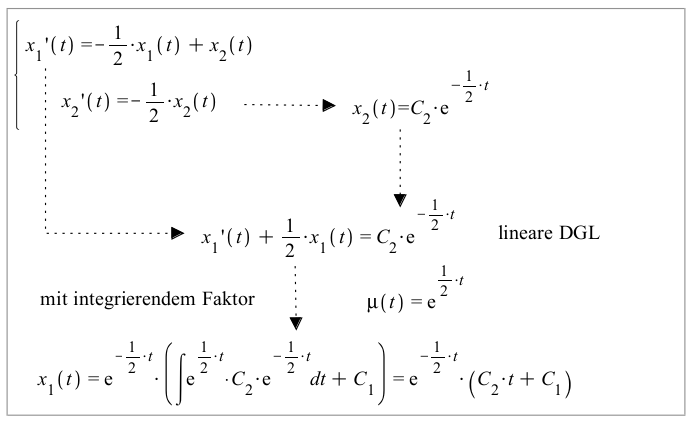
\includegraphics[width=1.0\textwidth]{images/Entkoppeln.png}
\end{minipage}


\section{Kapitel 3}
%TODO by Hannes
\section{Kapitel 4}
%TODO
-Attraktor-Bereich\\
-Separatrizen\\
-Fast lineare Systeme/Jakobi-Matrix\\
-Konkurrenz-Modell\\
-Raeuber-Beute-Modell\\
-Periodische Loesungen und Grenzzyklen\\


\end{document}